\documentclass[11pt,a4paper,notitlepage]{report}
\usepackage[T1]{fontenc}
\usepackage[utf8]{inputenc}
\usepackage{lmodern,microtype}
\usepackage[margin=1.1in,headheight=14pt]{geometry}
\usepackage{amsmath,amssymb,amsthm}
\usepackage{booktabs,array,longtable,graphicx,xurl}
\usepackage{xcolor}
\definecolor{linknavy}{RGB}{25,55,125}
\usepackage[colorlinks=true,linkcolor=linknavy,citecolor=linknavy,urlcolor=linknavy]{hyperref}
\usepackage{orcidlink}
\usepackage{fancyhdr}
\hypersetup{pdftitle={Directional Coupled Peak Penalties with Original Interval Rows},
pdfauthor={Felipe Santibáñez-Leal},pdfsubject={Directional group penalties and a registered negative computational result}}

\newtheorem{theorem}{Theorem}[chapter]
\newtheorem{proposition}[theorem]{Proposition}
\theoremstyle{remark}
\newtheorem{remark}[theorem]{Remark}
\DeclareMathOperator{\prox}{prox}
\DeclareMathOperator{\diag}{diag}
\DeclareMathOperator{\median}{median}
\newcommand{\R}{\mathbb{R}}
\newcommand{\pos}[1]{\left(#1\right)_{+}}
\newcommand{\norm}[1]{\left\lVert#1\right\rVert_{\infty}}

\newcommand{\doctype}{Technical report}
\newcommand{\docversion}{v0.02.001}
\newcommand{\docdate}{2 November 2026}
\newcommand{\versiondoi}{10.5281/zenodo.23885695}
\newcommand{\conceptdoi}{10.5281/zenodo.23875071}
\newcommand{\docrepo}{github.com/fsantibanezleal/CAOS\_SoftQP}
\newcommand{\headerblock}{%
\begin{center}
\fbox{\parbox{0.94\textwidth}{\small\raggedright
\textbf{\doctype} \quad$\cdot$\quad \docversion, \docdate \quad$\cdot$\quad Licence CC BY 4.0\\[2pt]
CAOS open-research programme \quad$\cdot$\quad directional coupled peak penalties\\[2pt]
Version DOI \href{https://doi.org/\versiondoi}{\texttt{\versiondoi}}\\[2pt]
Concept DOI (always latest) \href{https://doi.org/\conceptdoi}{\texttt{\conceptdoi}}\\[2pt]
Not peer reviewed. Source code, data and computational records:
\href{https://\docrepo}{\texttt{\docrepo}}
}}
\end{center}
\vspace{4pt}}

\title{Directional Coupled Peak Penalties\\with Original Interval Rows}
\author{Felipe Santib\'a\~nez-Leal\,\orcidlink{0000-0002-0150-3246}\\
\small CAOS open-research programme, Santiago, Chile}
\date{}
\pagestyle{fancy}
\fancyhf{}
\fancyhead[L]{\small CAOS Research \doctype}
\fancyhead[R]{\small Directional group peaks \textperiodcentered\ \docversion}
\fancyfoot[C]{\small \thepage}
\renewcommand{\headrulewidth}{0.4pt}
\fancypagestyle{plain}{\fancyhf{}\fancyhead[L]{\small CAOS Research \doctype}\fancyhead[R]{\small Directional group peaks \textperiodcentered\ \docversion}\fancyfoot[C]{\small \thepage}\renewcommand{\headrulewidth}{0.4pt}}
\fancypagestyle{titlepage}{\fancyhf{}\fancyfoot[C]{\small \thepage}\renewcommand{\headrulewidth}{0pt}}
% Numeric export from the reviewed summary; no new inference.
\newcommand{\PrimaryEstimate}{-212.449875}
\newcommand{\PrimaryLower}{-225.336618}
\newcommand{\PrimaryUpper}{-192.873759}
\newcommand{\PrimaryFailed}{9}
\newcommand{\PrimaryPopulation}{144}
\newcommand{\SummaryDigest}{c82bf30bb53c7c10d464fc446bd2b99ee774b581dbe3f4dced86194e1fe54c6d}
\newcommand{\DevelopmentAccepted}{879}
\newcommand{\DevelopmentAccuracyRejected}{0}
\newcommand{\DevelopmentIncompatible}{396}
\newcommand{\DevelopmentOracleFailed}{21}
\newcommand{\DevelopmentTimeout}{0}
\newcommand{\HeldoutAccepted}{2587}
\newcommand{\HeldoutAccuracyRejected}{6}
\newcommand{\HeldoutIncompatible}{1188}
\newcommand{\HeldoutOracleFailed}{105}
\newcommand{\HeldoutTimeout}{2}
\newcommand{\RobustnessAccepted}{201}
\newcommand{\RobustnessAccuracyRejected}{6}
\newcommand{\RobustnessIncompatible}{135}
\newcommand{\RobustnessOracleFailed}{144}
\newcommand{\RobustnessTimeout}{0}


\begin{document}
\maketitle
\thispagestyle{titlepage}
\headerblock
\begin{abstract}
Directional group peaks price the largest weighted departure across selected interval
constraints. We derive the box slack-elimination and diagonal-metric proximal identities
for coordinate-contraction-monotone penalties, specialize them to directional
linear--quadratic group peaks, and describe a native implementation that retains the
original interval-row system. Directional row splitting and compact epigraphs already
express the same objective; weighted threshold operations and relaxed splitting also
have established precedents. The empirical question is whether preserving the original
rows reduces complete repeated-forecast computation time against these alternatives.
A prospectively registered study retains 210 synthetic instances and 7770 observations
across development, heldout and robustness splits. The primary population comprises
all \PrimaryPopulation{} heldout instances in six seed clusters, with 32 forecasts and
three measured repetitions per method and instance. The median paired reduction score is
\PrimaryEstimate\%, with a 95\% seed-cluster interval of
$[\PrimaryLower\%,\PrimaryUpper\%]$, and \PrimaryFailed{} failed pairs retained under
the prescribed scoring rule. The registered 10\% improvement is not established.
All returned candidate frames satisfy their applicable original-space numerical
criteria; iteration limits, unsuccessful common oracles and timeouts remain part of
the result. The findings concern synthetic problems on one nonreserved host and do not
establish a general speed advantage, operational safety or historical algorithmic priority.
\end{abstract}

\chapter{Problem, formulation and related work}
\section{Directional interval preferences}
Soft constraints represent priced departures from operational preferences. They do not
make immutable physical limits optional. A shared group peak couples the departures
of several rows: increasing the largest departure can change how a solver allocates
corrections to every row in that group. Unequal upper and lower scales express
different consequences for the two directions.

Let $P\in\R^{n\times n}$ be symmetric positive semidefinite, $q\in\R^n$ finite,
and $A\in\R^{m\times n}$ sparse. Lower and upper interval endpoints may be absent.
Disjoint index sets $I_g$ specify soft groups; the remaining rows form the hard set
$\mathcal H$. Group prices satisfy $a_g,b_g\geq0$, and the finite directional scales
$c_{U,i},c_{L,i}$ are strictly positive. With $t_+=\max(t,0)$, define
\begin{equation}\label{eq:peak}
M_g(z)=\max\left\{0,\ \max_{i\in I_g}c_{U,i}(z_i-u_i)_+,\
                         \max_{i\in I_g}c_{L,i}(\ell_i-z_i)_+\right\}.
\end{equation}
An absent side contributes no departure. The optimization problem is
\begin{align}\label{eq:problem}
\underset{x\in\R^n}{\operatorname{minimize}}\quad&
\tfrac12 x^\top P x+q^\top x+
 \sum_g\left(a_g M_g(Ax)+\tfrac12 b_g M_g(Ax)^2\right),\\
\text{subject to}\quad& \ell_i\leq A_i x\leq u_i\quad(i\in\mathcal H).\nonumber
\end{align}
The constraints in $\mathcal H$ remain hard. A group with $a_g=b_g=0$ has zero
penalty and is free, rather than hard. Invalid intervals, overlapping or empty groups,
nonpositive directional scales and negative curvature are refused by the interface.

\section{Equivalent formulations and attribution}
Schwan, Lew and Plancher develop generalized slack projections for soft-constrained
quadratic programs without increasing the principal system dimensions~\cite{gsp}.
The relation between orthant behavior and coordinatewise monotonicity is established
in convex analysis~\cite{orthant}; proximal operations and relaxed splitting are also
established tools~\cite{prox,admm}. Weighted threshold and projection algorithms have
substantial prior work~\cite{weighted}. These precedents preclude identifying
directional expressibility, a threshold calculation or relaxation alone as a new method.

Directional row splitting replaces an original row by
\begin{equation}\label{eq:rowsplit}
c_{U,i}A_i x\leq c_{U,i}u_i,\qquad
-c_{L,i}A_i x\leq-c_{L,i}\ell_i,
\end{equation}
omitting absent sides. The symmetric upper departure peak of these rows equals
\eqref{eq:peak}. Alternatively, one nonnegative epigraph variable $t_g$ per active
group gives the exact compact formulation
\begin{align}\label{eq:epigraph}
\underset{x,t}{\operatorname{minimize}}\quad&
\tfrac12 x^\top P x+q^\top x+\sum_g(a_g t_g+\tfrac12 b_g t_g^2),\\
\text{subject to}\quad& t_g\geq0,\quad
 c_{U,i}(A_i x-u_i)\leq t_g,\quad
 c_{L,i}(\ell_i-A_i x)\leq t_g\quad(i\in I_g),\nonumber
\end{align}
together with the original hard rows. Thus the computational comparison must retain
both compact epigraphs and directional row splitting. It tests the cost of an
original-row implementation, rather than the ability to express the objective.

\chapter{Slack elimination and the proximal calculation}
\section{An exact box identity}
Let $C$ be a nonempty closed box, and let $\Psi$ be a proper closed convex
nonnegative function with $\Psi(0)=0$. Write $\Pi_C$ for Euclidean box projection.
The contraction property is
\begin{equation}\label{eq:contraction}
\Psi(Dw)\leq\Psi(w),\qquad
D=\diag(d_i),\quad 0\leq d_i\leq1.
\end{equation}
It permits unequal prices on the two rays of a coordinate; it does not require
sign symmetry. Define the eliminated interval cost by
\begin{equation}\label{eq:infimal}
g_C(z)=\inf_{s\in C}\Psi(z-s).
\end{equation}

\begin{theorem}[Box reduction]\label{thm:box}
Property~\eqref{eq:contraction} is necessary and sufficient for the identity
\begin{equation}\label{eq:box}
g_C(z)=\Psi\bigl(z-\Pi_C(z)\bigr)
\end{equation}
to hold for every nonempty closed box $C$ and every $z$.
\end{theorem}
\begin{proof}
For any $s\in C$, set $r=z-\Pi_C(z)$. If $z_i>u_i$, then $z_i-s_i\geq r_i>0$;
if $z_i<\ell_i$, then $z_i-s_i\leq r_i<0$. If $z_i$ is inside its interval,
$r_i=0$. Consequently $r=D(z-s)$ for a diagonal contraction $D$.
Property~\eqref{eq:contraction} gives $\Psi(r)\leq\Psi(z-s)$, and choosing
$s=\Pi_C(z)$ attains equality.

Conversely, fix $w$ and a diagonal contraction $D$. Choose each interval to have
endpoints $-w_i$ and $-d_iw_i$, in increasing order, and set $z=0$. The nearest-box
residual is $Dw$, whereas $-w\in C$. Identity~\eqref{eq:box} then implies
$\Psi(Dw)\leq\Psi(w)$.
\end{proof}
The infimal-convolution representation makes $g_C$ convex, and the continuous residual
map in~\eqref{eq:box} gives lower semicontinuity. Corrective slack has the opposite
sign to violation residual: in $z+\xi\in C$, its cost is $\Phi(\xi)=\Psi(-\xi)$.

\section{Positive diagonal metrics}
For $H=\diag(h_i)\succ0$, define
\begin{equation}\label{eq:metricprox}
\prox_f^H(v)=\underset{z}{\arg\min}\left\{f(z)+\tfrac12(z-v)^\top H(z-v)\right\}.
\end{equation}
The metric is fixed during this calculation.
\begin{proposition}[Translated residual proximal map]\label{prop:prox}
Under the preceding assumptions,
\begin{equation}\label{eq:proxidentity}
\prox_{g_C}^H(v)=\Pi_C(v)+\prox_{\Psi}^H\bigl(v-\Pi_C(v)\bigr).
\end{equation}
\end{proposition}
\begin{proof}
Put $p=\Pi_C(v)$ and clip each candidate coordinate to the segment with endpoints
$p_i$ and $v_i$. Diagonality of $H$ makes this clipping nonincreasing for the squared
distance from $v$. The clipped point's box residual is a diagonal contraction of
the original residual, so its penalty cannot increase either. An optimum may
therefore be sought on that product of segments.

On this set, write $z=p+w$ and $r=v-p$. Its box residual equals $w$, so the
objective becomes $\Psi(w)+\tfrac12(w-r)^\top H(w-r)$. The unconstrained residual
proximal minimizer lies on the same segments between $0$ and $r$: coordinate
clipping reduces both its distance from $r$ and its penalty. Hence restricting to
those segments does not alter that minimum, proving~\eqref{eq:proxidentity}.
\end{proof}
This is an exact convex-analytic statement. It supplies neither a finite-precision
error bound nor an elapsed-time improvement.

\section{Directional peak threshold}
For one group, set
\begin{equation}\label{eq:residualpeak}
\Psi(w)=aM(w)+\tfrac12 bM(w)^2,\qquad
M(w)=\max_i\{c_{U,i}(w_i)_+,c_{L,i}(-w_i)_+\}.
\end{equation}
This penalty satisfies~\eqref{eq:contraction}. On the residual segments let $c_i$
be $c_{U,i}$ for $r_i\geq0$ and $c_{L,i}$ for $r_i<0$. For a prescribed peak
$t\geq0$, coordinate projection gives
\begin{equation}\label{eq:wthreshold}
w_i(t)=\operatorname{sign}(r_i)\min\{|r_i|,t/c_i\}.
\end{equation}
The remaining scalar convex minimization is
\begin{equation}\label{eq:scalar}
\underset{t\geq0}{\operatorname{minimize}}\quad
F(t)=at+\tfrac12bt^2+\tfrac12\sum_i h_i\bigl(|r_i|-t/c_i\bigr)_+^2.
\end{equation}
Sorting the breakpoints $c_i|r_i|$ in descending order identifies an active prefix
$S(t)=\{i:c_i|r_i|>t\}$. On an interval with that active set, $F'(t)=0$ gives
\begin{equation}\label{eq:tthreshold}
t=\frac{\sum_{i\in S(t)}h_i|r_i|/c_i-a}
        {b+\sum_{i\in S(t)}h_i/c_i^2}.
\end{equation}
The formula is evaluated only with a positive denominator. Empty active sets are
handled by the scalar objective and interval endpoints, never by division by zero.
The consistent interval and the endpoint $t=0$ determine the minimizer. If the right
derivative at zero is nonnegative, the minimizer is zero. If $a=b=0$, the proximal
map returns the unchanged residual directly. The implementation uses finite local
floating-point spacing at threshold boundaries and refuses nonrepresentable
arithmetic; an absolute tolerance floor would not establish invariance to units.

\section{Joint conjugates and original-space checks}
Define the joint directional dual quantity
\begin{equation}\label{eq:dualbudget}
L_g(y)=\sum_{i\in I_g}\left(\frac{(y_i)_+}{c_{U,i}}+
                                      \frac{(-y_i)_+}{c_{L,i}}\right).
\end{equation}
Maximizing $y^\top w$ at fixed peak $M(w)\leq t$ gives $tL_g(y)$. Taking the
scalar conjugate therefore yields
\begin{equation}\label{eq:conjugate}
\Psi_g^*(y)=
\begin{cases}
\dfrac{(L_g(y)-a_g)_+^2}{2b_g},&b_g>0,\\[4pt]
0,&b_g=0,\ L_g(y)\leq a_g,\\
+\infty,&b_g=0,\ L_g(y)>a_g.
\end{cases}
\end{equation}
This is a group budget, rather than independent coordinate caps. The box support
function $\sigma_C$ is also required:
\begin{equation}\label{eq:dualkkt}
g_C^*(y)=\sigma_C(y)+\Psi^*(y),\qquad Px+q+A^\top y=0.
\end{equation}
A positive multiplier requires a finite upper side and a negative multiplier a
finite lower side. Numerical acceptance checks raw and repaired stationarity,
bounded dual repair, each group's absolute normalized Fenchel gap and each hard
row's complementarity separately. A negative approximate hard-row gap cannot cancel
an incorrect soft subgradient. The signed aggregate gap remains diagnostic.

\chapter{Native splitting, scaling and comparison formulations}
\section{Fixed-metric relaxed splitting}
Use consensus variables $u=(x,z)$ and $v$, and define
\begin{equation}\label{eq:FG}
F(x,z)=\tfrac12x^\top Px+q^\top x+\iota_{\{z=Ax\}}(x,z),
\end{equation}
with $G(v)$ containing the hard intervals and soft costs. The fixed block metric
is $\mathcal M=\diag(S,H)$, where $S\succ0$ and $H\succ0$. In particular,
\begin{equation}\label{eq:graphsystem}
P+S+A^\top H A\succ0.
\end{equation}
With scaled dual $d$, the four relaxed updates are
\begin{align}\label{eq:relaxed}
u^{k+1}&=\prox_F^{\mathcal M}(v^k-d^k),\\
h^{k+1}&=\alpha u^{k+1}+(1-\alpha)v^k,\nonumber\\
v^{k+1}&=\prox_G^{\mathcal M}(h^{k+1}+d^k),\nonumber\\
d^{k+1}&=d^k+h^{k+1}-v^{k+1}.\nonumber
\end{align}
Let $R_F=2\prox_F^{\mathcal M}-I$, $R_G=2\prox_G^{\mathcal M}-I$ and $s=v+d$.
After a complete step $v=\prox_G^{\mathcal M}(s)$, so substitution gives
\begin{equation}\label{eq:DR}
s^{k+1}=(1-\alpha/2)s^k+(\alpha/2)R_F R_G(s^k),\qquad0<\alpha<2.
\end{equation}
Whitening the fixed metric reduces this to the usual reflected-proximal setting.
For proper closed convex $F$ and $G$, exact proximal subproblems and a finite
saddle point, the reflected composition is nonexpansive
and the strict interior relaxation is averaged. The standard fixed-point and shadow
arguments give convergence~\cite{prox,admm}. The endpoints zero and two are excluded;
the penalty prices acquire no $\alpha$ factor. No new convergence-rate theorem is asserted.

The public native implementation fixes a finite scalar $\alpha\in(0,2)$, defaults to
1.6 and uses direct linear solves. It rejects adaptive penalty updates, automatic
OSQP scaling, polishing, directional sensitivities and directional code generation.
Its supported implementation scope is narrower than the diagonal-metric identity.

\section{Normalization and workspace invariants}
For positive diagonal $D$, consistent row normalization is
\begin{align}\label{eq:scaling}
\bar A&=DA,&\bar\ell&=D\ell,&\bar u&=Du,&\bar c&=c/D,\\
y&=D\bar y,& H_{\rm physical}&=D\bar H D.\nonumber
\end{align}
The bounds must scale with the rows. Setup selects
$D_i=\max(c_{L,i},c_{U,i})$ on soft rows and $D_i=1$ on hard rows. This selects the
corresponding physical metric; it does not preserve the former unscaled-penalty
iteration trajectory. The metric, relaxation, $P$, $A$, group membership, prices,
directional scales, finite-side pattern and hard-row penalty classification remain
fixed within a workspace. The forecast sequence updates $q$ and interval bounds.

Numerical failures clear purported solutions and diagnostics. A quadratic group
blocks finite-side violating recession directions. The unboundedness implementation
conservatively requires exactly zero computed $Pd$; ambiguous directions remain
unresolved. Ambiguous coupled semidefinite blocks larger than the exact
32-variable certification limit are unsupported rather than silently regularized.

\section{Nine registered profiles}
Table~\ref{tab:profiles} lists the complete comparison set. All five OSQP-style
profiles use $\alpha=1.6$, absolute and relative tolerances $10^{-8}$, at most
200000 iterations and no polishing. Fixed profiles additionally set $\rho=0.1$,
$\sigma=10^{-6}$, no adaptive penalty and no automatic scaling. The native profile
uses its explicit row normalization. Default epigraph and row-split profiles use
adaptive penalty and ten scaling iterations.
DAQP profiles use absolute tolerance $10^{-8}$ and a 200000-iteration limit;
proximal profiles use $\eta_{\rm prox}=10^{-10}$. Direct DAQP requires a
positive-definite augmented epigraph Hessian. The pinned row-split generalized
projection supports the native linear infinity penalty, so squared peaks are
declared incompatible. Proximal DAQP preserves the unchanged semidefinite or linear
objective. In DAQP 0.10.3, one-shot zero-Hessian and persistent Model policies are
distinct. Flags 4 and 5 supply candidates only; independent checks must still
accept them~\cite{daqp}. Unsupported objectives remain explicit cells.

\begin{table}[htbp]\centering\small
\caption{The registered methods and their distinct policies.}\label{tab:profiles}
\begin{tabular}{@{}p{0.31\textwidth}p{0.62\textwidth}@{}}\toprule
Profile & Formulation and controls\\\midrule
\texttt{native} & Original-row directional group projection; fixed metric.\\
\texttt{epigraph-default} & Stock OSQP compact epigraph; default adaptation/scaling.\\
\texttt{epigraph-fixed} & Stock OSQP compact epigraph; fixed controls.\\
\texttt{row-split-default} & Directional row-split generalized slack projection; default controls.\\
\texttt{row-split-fixed} & Directional row-split generalized slack projection; fixed controls.\\
\texttt{daqp-direct} & Direct non-proximal compact epigraph.\\
\texttt{daqp-prox-auto} & Proximal epigraph; $\epsilon_{\rm prox}=-10^{-6}$; one-shot LP policy.\\
\texttt{daqp-prox-forced} & Proximal epigraph; $\epsilon_{\rm prox}=1$; one-shot LP policy.\\
\texttt{daqp-lp-model} & Proximal epigraph; $\epsilon_{\rm prox}=-10^{-6}$; persistent LP model policy.\\\bottomrule
\end{tabular}
\end{table}

\chapter{Experimental design and numerical acceptance}
\section{Synthetic inputs and complete populations}
The study comprises 48 development instances, 144 heldout instances and 18 robustness
instances. Each instance supplies 32 forecasts. Every heldout seed has sixteen sparse
and eight thermal cells. Sparse cells use $n=32$ or $96$, group size eight,
pre-zeroing geometric diagonal spans one or 1000, positive-definite or semidefinite
base curvature and $b_g=0$ or 1. Hard coordinate bounds retain bounded objectives.
For semidefinite $P$, the full-matrix condition is infinite; the span label describes
the diagonal before zeroing and is not a finite Hessian condition number.

Thermal cells have two independent zones, horizons of twelve or twenty-four one-hour
intervals, explicit temperatures and heater-energy inputs. Initial conditions,
dynamics and heater limits remain hard. One directional comfort peak is shared over
each zone's horizon. The conventional horizon organization follows the standard
quadratic-control formulation~\cite{mpc}. For each zone the dynamics have the form
\begin{equation}\label{eq:thermal}
T_{k+1}=aT_k+bQ_k+(1-a)T_{{\rm outside},k}.
\end{equation}
Temperature is in degrees Celsius, $Q_k$ is heater energy in kWh per interval, and
the objective uses synthetic currency. Retention, gains, weather and prices are
authored synthetic values. These are repeated forecasts, not building measurements
or independently evolving closed-loop policies.

Robustness separately includes zero-Hessian base cases and a $10^8$ diagonal span,
with eighteen instances over three seeds. A zero base Hessian with $b_g>0$ still
produces a quadratic epigraph objective and is not a pure linear program. Development
and robustness are descriptive and cannot replace the heldout endpoint.

\section{Measured operation and process supervision}
One timed observation includes owned validation, formulation construction and
factorization, every forecast update and solve, physical recovery and independent
checks. Canonical generation, process/library startup and serialization are excluded
symmetrically. Competing compiled libraries are preloaded before the inner timer.
Each observation has a fresh supervised process, with workspace reuse only across
its own 32 forecasts. One warmup and three measured repetitions are retained per
method and instance.

The 30-second worker wall limit includes startup and serialization. Split supervision
has a four-hour wall limit and a sampled 4-GiB current/high-water resident-memory
limit. These limits do not reserve CPU or memory. Unrelated host work remains present.
The source, dependency map and public SDK/native-wheel identity are registered before
execution. No failed case is retuned, reseeded, retried or replaced.

\section{Accuracy in original coordinates}
Candidate frames require hard-row error at most $10^{-6}$ in the declared physical
units; raw and repaired normalized stationarity, maximum local absolute normalized
Fenchel gap, joint dual-budget error and normalized common-oracle objective discrepancy
at most $10^{-6}$; and normalized dual repair at most $10^{-7}$. Every forecast must
pass. The common stock-OSQP compact-epigraph oracle uses absolute and relative
tolerances $10^{-10}$, 200000 iterations and an external $10^{-7}$ criterion.

For example, stationarity uses the worse of the raw and repaired multiplier values of
\begin{equation}\label{eq:stationarity}
\frac{\norm{Px+q+A^\top y}}
     {\max\{1,\norm{Px},\norm{q},\norm{A^\top y}\}}.
\end{equation}
Objective discrepancy is normalized by $\max(1,|f_{\rm oracle}|)$. A group's Fenchel
denominator is $\max(1,|\Psi_g|,|\sigma_{C_g}(y_g)|,|y_g^\top A_gx|)$; hard-row
denominators are $\max(1,|y_i\,\mathrm{bound}_i|,|y_i(Ax)_i|)$. Dual repair uses
$\max(1,\norm{y})$, and linear joint-budget excess uses $\max(1,L_g,a_g)$.
Nonfinite products are rejected before normalization. Bounded repair does not
retroactively make the original multiplier an exact member of the dual domain.

\section{Primary inference}
For instance $j$ and profile $m$, let
\begin{equation}\label{eq:timemedian}
T_{j,m}=\median_{r=1,2,3}T_{j,m,r}.
\end{equation}
If every compatible measured observation succeeds, define the paired score
\begin{equation}\label{eq:reduction}
R_j=1-\frac{T_{j,\mathrm{native}}}
 {\min_{m\ne\mathrm{native},\ m\ \mathrm{compatible}}T_{j,m}},
\end{equation}
with lexical baseline tie-breaking. Any missing or unsuccessful compatible measured
observation instead assigns $R_j=-1$ to the pair and prevents qualification.
All 144 instances remain in the population; there is no successful-only denominator.

The bootstrap resamples six whole seeds with replacement, pools their complete
24-instance vectors and takes the median. It uses 10000 resamples and NumPy's linear
2.5th/97.5th percentile limits. The registered prediction requires a median reduction
of at least 10\%, a strictly positive lower confidence limit and zero failed pairs.
The interval concerns the registered seed clusters and observed workload, not
universal hardware performance.

\chapter{Results and retained failures}
\section{Primary outcome}
The median paired score is \PrimaryEstimate\%, with a 95\% seed-cluster interval
from $\PrimaryLower\%$ to $\PrimaryUpper\%$ and \PrimaryFailed{} failed pairs out of
\PrimaryPopulation{}. The registered prediction fails all three conditions: its
estimate is below 10\%, its lower confidence limit is negative, and unsuccessful
pairs remain. The score combines observed relative times with the prescribed
failed-pair value; it is not a uniform runtime multiplier for every case.

\begin{figure}[htbp]\centering
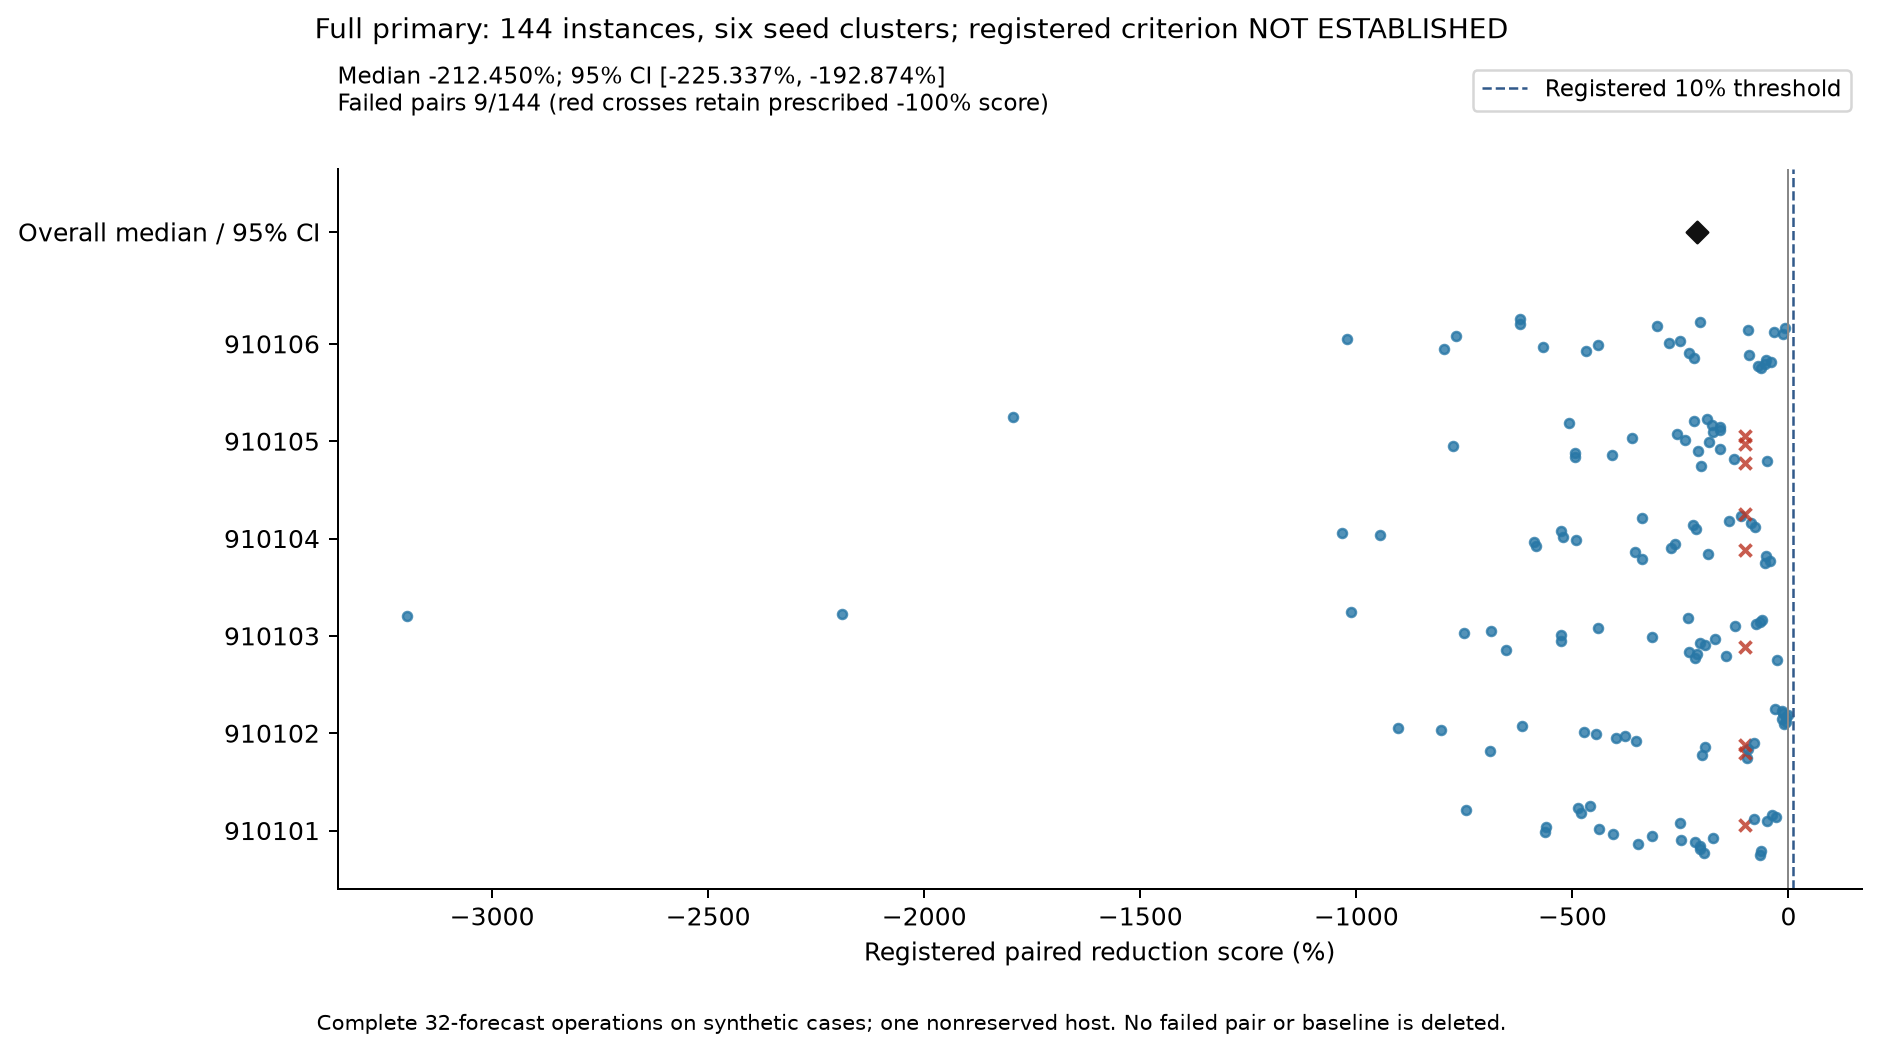
\includegraphics[width=\textwidth]{results/summary/primary-full-population.png}
\caption{All 144 registered paired scores, including the nine unsuccessful pairs at
their prescribed $-100\%$ score. That value is a failure policy, distinct from
observed negative runtime reductions. The full plotted range retains extreme values.}
\label{fig:primary}
\end{figure}

\section{Every measured state}
The complete raw journals contain 7770 observations, including warmups and common
oracles. Table~\ref{tab:states} separates the 5670 measured method observations.
There are 3667 accepted, twelve accuracy-rejected, 1719 incompatible, 270 dependent
oracle-failed and two timed-out measured observations. The twelve accuracy-rejected
batches contain backend iteration limits without returned primal or dual vectors;
they are not inaccurate completed KKT solutions.
\begin{table}[htbp]\centering
\caption{Measured method observations; no state is removed from the inventory.}
\label{tab:states}
\begin{tabular}{@{}lrrr@{}}\toprule
State & Development & Heldout & Robustness\\\midrule
Accepted & \DevelopmentAccepted & \HeldoutAccepted & \RobustnessAccepted\\
Accuracy-rejected & \DevelopmentAccuracyRejected & \HeldoutAccuracyRejected & \RobustnessAccuracyRejected\\
Incompatible & \DevelopmentIncompatible & \HeldoutIncompatible & \RobustnessIncompatible\\
Oracle-failed & \DevelopmentOracleFailed & \HeldoutOracleFailed & \RobustnessOracleFailed\\
Timeout & \DevelopmentTimeout & \HeldoutTimeout & \RobustnessTimeout\\\bottomrule
\end{tabular}
\end{table}
\begin{figure}[htbp]\centering
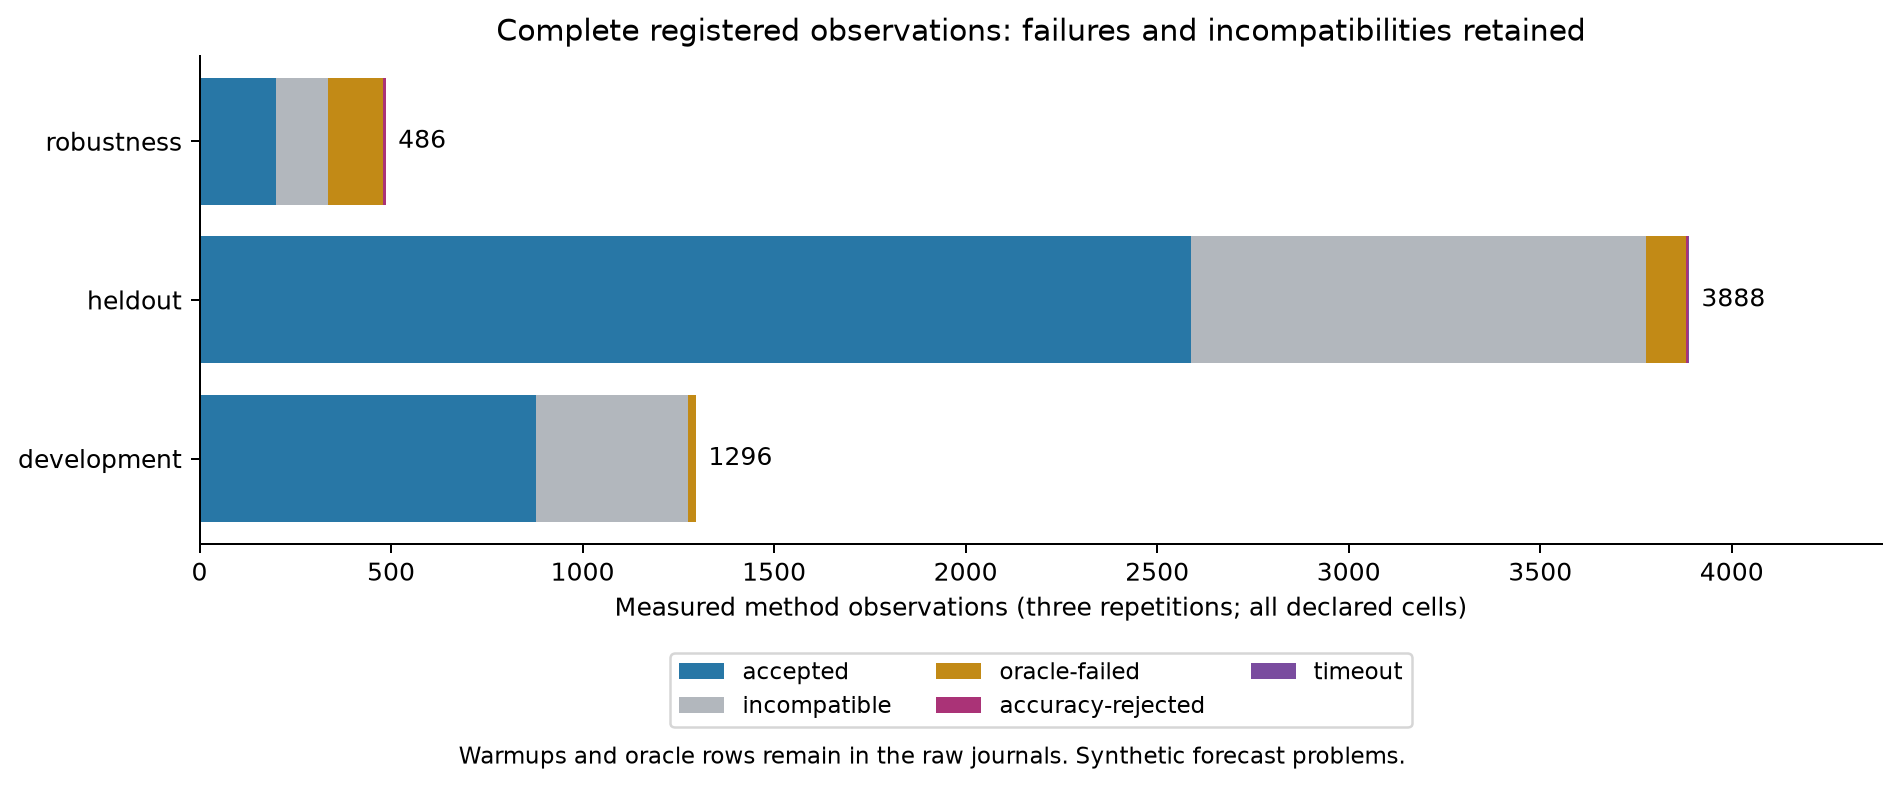
\includegraphics[width=\textwidth]{results/summary/observation-states.png}
\caption{Every measured state in the three splits. Warmups and common-oracle records
remain in the full journals and are not added to the measured-state bars.}
\label{fig:states}
\end{figure}

\section{Failure taxonomy and numerical verification}
Development has one unsuccessful common oracle, \texttt{development-0014} at frame
13, and 21 dependent measured oracle-failed observations. Independent recomputation
checks 39021 returned candidate frames, including thirteen valid prefix frames of
that unsuccessful oracle; the automatic accepted-batch consumer checks 39008 frames.

Heldout has five common-oracle iteration limits: \texttt{heldout-0030}/frame 0,
\texttt{0054}/22, \texttt{0078}/0, \texttt{0106}/3 and \texttt{0110}/3, all with
the \texttt{heldout-} prefix. They produce 105 dependent measured oracle-failed
observations. The six accuracy-rejected batches are \texttt{row-split-default} on
\texttt{heldout-0014}, frame 3, and \texttt{heldout-0026}, frame 22, in all three
measured repetitions. Each reaches status 7 at 200000 iterations without candidate
vectors; warmups fail identically. Timeouts occur for \texttt{native} on
\texttt{heldout-0095}, repetition index 1, and \texttt{daqp-prox-forced} on
\texttt{heldout-0097}, repetition index 2. Indices are zero-based. Five oracle cases,
two row-split cases and two timeout cases account for nine failed primary pairs.

Independent heldout recomputation checks 115124 returned candidate frames, all
passing their respective original-space criteria. This includes 248 valid frames
from rejected method batches and 28 valid prefixes of failed oracles in addition
to 114848 accepted-batch frames. The two counts have different scopes and must not
be added together. A killed worker supplies no completed numerical conclusion.

Robustness has six unsuccessful common oracles: \texttt{robustness-0000}/frame 21,
\texttt{0002}/15, \texttt{0006}/0, \texttt{0008}/4, \texttt{0012}/0 and
\texttt{0014}/13, all with the \texttt{robustness-} prefix. The six measured
accuracy-rejected batches are \texttt{native} and \texttt{epigraph-fixed} on
\texttt{robustness-0003}, each over all three repetitions. Status 7 occurs at frames
1, 24 and 25 after 200000 iterations, without candidate vectors; warmups behave
identically. Independent recomputation checks 9245 returned candidate frames, all
passing, versus 8960 accepted-batch frames. The six oracle limits produce 144
dependent measured oracle-failed observations.

Across all splits, 163390 returned candidate frames satisfy their applicable checks;
44 noncandidate backend-limit frames remain separate. An unsuccessful common oracle
does not by itself prove a candidate algorithm wrong or slower. It makes the
registered pair unsuccessful. No oracle substitution, failure deletion or retry
changes the primary outcome.

\chapter{Interpretation, limitations and conclusions}
The mathematical identities explain how directional group peaks can retain original
interval rows. Exact epigraphs and directional row splitting already express that
same objective. Preserving principal dimensions alone therefore does not establish
a computational advantage. The complete-operation measurements refute the registered
runtime prediction for the observed workload.

The earlier separable study~\cite{separable} is a different 456-instance computation.
Its median reduction was 0.499839\%, with a 95\% interval of
$[-3.291967\%,3.944835\%]$, which also failed its 10\% prediction. These populations,
endpoints and penalty families cannot be pooled into an improvement claim.

The current results are limited to authored synthetic sparse problems and thermal
forecasts, nine registered profiles, three measured repetitions and six primary
seed clusters on one nonreserved Windows host. They are not field energy savings,
closed-loop safety evidence or a universal runtime comparison. Factorization costs
and allocations were not isolated causal effects. Conservative numerical refusal,
iteration limits and process supervision are part of the reported behavior.

The fixed-metric splitting argument assumes a finite saddle point and does not cover
every adaptive implementation. Finite floating-point arithmetic needs separate
numerical checks. Larger ambiguous semidefinite cases outside the certification
scope remain unsupported. Neither the derivations nor the tests establish global
algorithmic novelty. The public engine is an engineering distribution, not a
certificate of operational suitability.

The contribution is an inspectable original-row directional implementation, its
bounded mathematical formulation and a reproducible negative comparison. The
registered 10\% speed improvement is not established. Any future computational
prediction requires its own justified protocol rather than a changed interpretation
of these retained observations.

\section*{Data and code availability}
The full synthetic inputs, original-space oracle/method journals, failures, warmups,
CSV, protocol and registered source snapshots are available in the supporting
dataset~\cite{dataset}. Its ZIP SHA256 is
\url{45b4eceda69f80a30a4ce349d0e9baefacace0de394fe315f3c392260ea8d418}.
The scientific source is commit
\url{246bf87e690f4d010494c556e2021d311d587422} of
\url{https://github.com/fsantibanezleal/CAOS_SoftQP}.
The independent engine source is
\url{https://github.com/fsantibanezleal/CAOS_SoftQP_Engine}; the study consumes
\texttt{softqp==0.2.0} from \url{https://pypi.org/project/softqp/0.2.0/}.
No external operational dataset or private records are needed. Source-code licenses
remain separate from the text license. The compiled document's source and build
instructions are included in the public repository.

\section*{Declaration of generative AI use}
Generative AI tools were used for mathematical development, software implementation,
document preparation and independent verification assistance. The author is responsible for reviewing and verifying all content and takes full
responsibility for the work.

\begin{thebibliography}{9}
\bibitem{gsp} R. Schwan, T. Lew and B. Plancher.
Efficient ADMM for Soft-Constrained Quadratic Programs via Generalized Slack Projections.
2026. \url{https://arxiv.org/abs/2610.35631}.
\bibitem{orthant} J.-P. Chancelier and M. de Lara.
Orthant-Strictly Monotonic Norms, Generalized Top-$k$ and $k$-Support Norms and the
$\ell_0$ Pseudonorm. \emph{Journal of Convex Analysis}, 30, 2023.
\url{https://arxiv.org/abs/2001.10441v3}.
\bibitem{prox} N. Parikh and S. Boyd. Proximal Algorithms.
\emph{Foundations and Trends in Optimization}, 1(3):123--231, 2014.
\url{https://web.stanford.edu/~boyd/papers/prox_algs.html}.
\bibitem{admm} S. Boyd, N. Parikh, E. Chu, B. Peleato and J. Eckstein.
Distributed Optimization and Statistical Learning via the Alternating Direction
Method of Multipliers. \emph{Foundations and Trends in Machine Learning},
3(1):1--122, 2011.
\url{https://web.stanford.edu/~boyd/papers/admm_distr_stats.html}.
\bibitem{weighted} G. Perez, S. Ament, C. Gomes and M. Barlaud.
Efficient projection algorithms onto the weighted $\ell_1$ ball.
\emph{Artificial Intelligence}, 306:103683, 2022.
\url{https://doi.org/10.1016/j.artint.2022.103683}.
\bibitem{daqp} DAQP contributors. Parameters and exit flags.
\url{https://darnstrom.github.io/daqp/parameters/}.
\bibitem{mpc} OSQP contributors. Model predictive control formulation.
\url{https://osqp.org/docs/examples/mpc.html}.
\bibitem{separable} F. Santib\'a\~nez-Leal.
Side-Specific Soft Constraints in Quadratic Programming. Technical report, 2026.
\url{https://doi.org/10.5281/zenodo.23851660}.
\bibitem{dataset} F. Santib\'a\~nez-Leal.
Directional coupled peak study: registered synthetic inputs and complete execution
evidence. Dataset, 2026. \url{https://doi.org/10.5281/zenodo.23875194}.
\end{thebibliography}
\end{document}
